\subsection{UC2: Configurazione della connessione tra rete bayesiana e sorgente dati}
\hypertarget{UC2}{}
\begin{figure} [H]
	\centering
	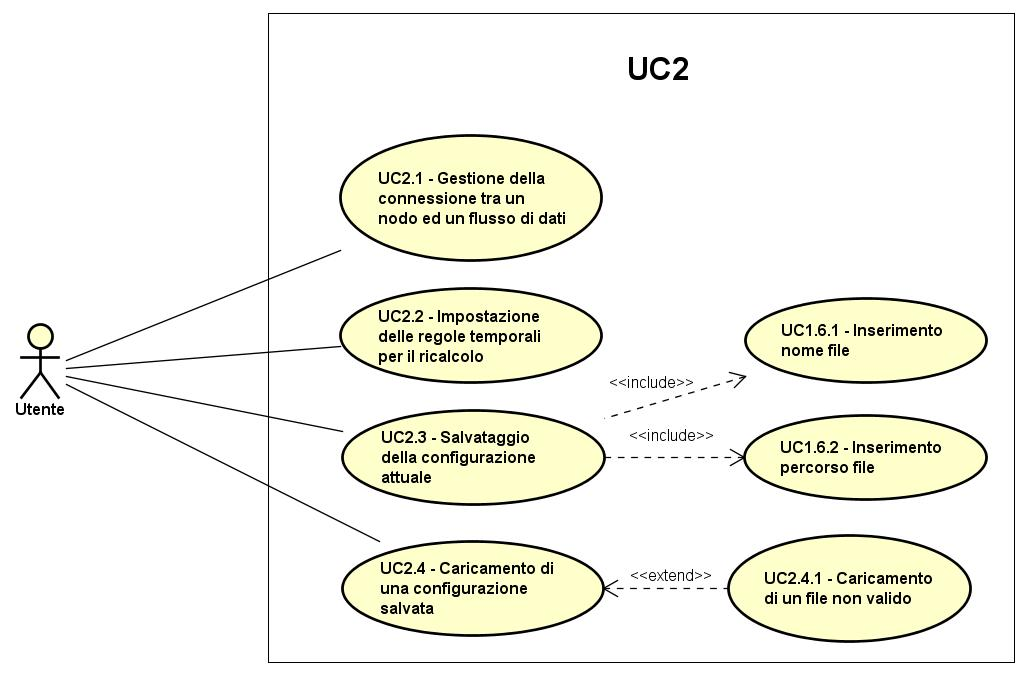
\includegraphics[scale=0.45]{Img/UC2}
	\caption{UC2: Configurazione della connessione tra rete bayesiana e sorgente dati}\label{}
\end{figure}
\begin{itemize}
	\item \textbf{Attori}: Utente;
	\item \textbf{Scopo e descrizione}: L'attore configura la connessione dei nodi della rete ai rispettivi flussi di dati provenienti dalla \gl{sorgente dati};
	\item \textbf{Precondizione}: È stata creata o caricata una rete bayesiana adeguata; Grafana riceve correttamente informazioni dalla sorgente dati;
	\item \textbf{Flusso principale degli eventi}:
	\begin{itemize}
		\item Gestione della connessione tra un nodo ed un flusso di dati (UC2.1);
		\item Impostazione delle regole temporali per il ricalcolo (UC2.2);
		\item Salvataggio della configurazione attuale (UC2.3);
		\item Caricamento di una configurazione salvata (UC2.4).
	\end{itemize}
	\item \textbf{Postcondizione}: La connessione tra la rete bayesiana e la sorgente dati è configurata correttamente.
\end{itemize}

\subsection{UC2.1: Gestione della connessione tra un nodo ed un flusso di dati}
\hypertarget{UC2.1}{}
\begin{figure} [H]
	\centering
	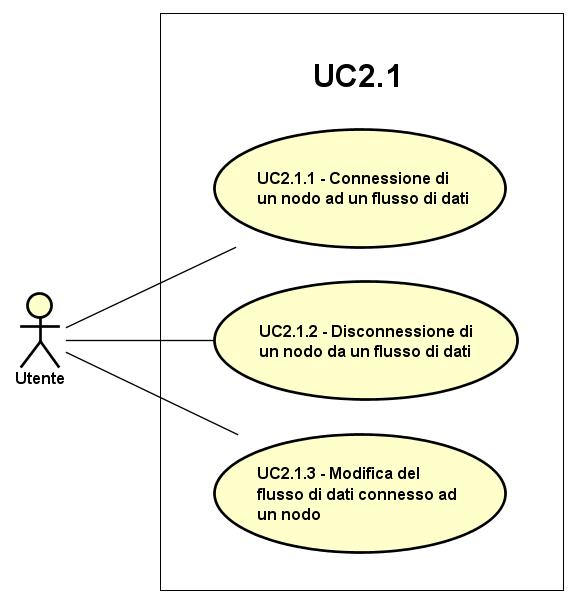
\includegraphics[scale=0.45]{Img/UC2-1}
	\caption{UC2.1: Gestione della connessione tra un nodo ed un flusso di dati}\label{}
\end{figure}
\begin{itemize}
	\item \textbf{Attori}: Utente;
	\item \textbf{Scopo e descrizione}: L'attore modifica il modo in cui un nodo è connesso ad un flusso di dati;
	\item \textbf{Precondizione}: L'attore ha selezionato un nodo della rete bayesiana;
	\item \textbf{Flusso principale degli eventi}:
	\begin{itemize}
		\item Connessione di un nodo ad un flusso di dati (UC2.1.1);
		\item Disconnessione di un nodo ad un flusso di dati (UC2.1.2);
		\item Modifica del flusso di dati connesso ad un nodo (UC2.1.3).
	\end{itemize}
	\item \textbf{Postcondizione}: Il nodo selezionato è connesso a, oppure disconnesso dal, flusso di dati designato.
\end{itemize}

\subsection{UC2.1.1: Connessione di un nodo ad un flusso di dati}
\hypertarget{UC2.1.1}{}
\begin{itemize}
	\item \textbf{Attori}: Utente;
	\item \textbf{Scopo e descrizione}: L'attore connette il nodo selezionato ad un flusso di dati;
	\item \textbf{Precondizione}: Il nodo selezionato non è connesso ad un flusso dati;
	\item \textbf{Postcondizione}: Il nodo selezionato è connesso al flusso di dati desiderato.
\end{itemize}

\subsection{UC2.1.2: Disconnessione di un nodo da un flusso di dati}
\hypertarget{UC2.1.2}{}
\begin{itemize}
	\item \textbf{Attori}: Utente;
	\item \textbf{Scopo e descrizione}: L'attore disconnette il nodo selezionato da un flusso di dati;
	\item \textbf{Precondizione}: Il nodo selezionato è connesso ad un flusso dati;
	\item \textbf{Postcondizione}: Il nodo selezionato è disconnesso dal flusso di dati.
\end{itemize}

\subsection{UC2.1.3: Modifica del flusso di dati connesso ad un nodo}
\hypertarget{UC2.1.3}{}
\begin{itemize}
	\item \textbf{Attori}: Utente;
	\item \textbf{Scopo e descrizione}: L'attore modifica il flusso di dati a cui un nodo è connesso;
	\item \textbf{Precondizione}: Il nodo selezionato è connesso ad un flusso dati diverso da quello desiderato;
	\item \textbf{Postcondizione}: Il nodo selezionato è connesso al flusso di dati desiderato.
\end{itemize}
\subsection{UC2.2: Impostazione delle regole temporali per il ricalcolo}
\hypertarget{UC2.2}{}
\begin{itemize}
	\item \textbf{Attori}: Utente;
	\item \textbf{Scopo e descrizione}: L'attore imposta le regole temporali per il ricalcolo delle probabilità della rete;
	\item \textbf{Precondizione}: È possibile inserire delle regole temporali;
	\item \textbf{Postcondizione}: L'attore inserisce le regole temporali desiderate.
\end{itemize}
\subsection{UC2.3: Salvataggio della configurazione attuale}

\hypertarget{UC2.3}{}
\begin{itemize}
	\item \textbf{Attori}: Utente;
	\item \textbf{Scopo e descrizione}: L'attore salva l'attuale configurazione della connessione della rete bayesiana al flusso dati in un file JSON per un futuro riutilizzo;
	\item \textbf{Precondizione}: La connessione tra rete bayesiana e sorgente dati è configurata nel modo desiderato, e il sistema ne permette il salvataggio in un file;
	\item \textbf{Postcondizione}: Viene salvato un file contenente la configurazione attuale.
\end{itemize}

\subsection{UC2.4: Caricamento di una configurazione salvata}
\hypertarget{UC2.4}{}
\begin{itemize}
	\item \textbf{Attori}: Utente;
	\item \textbf{Scopo e descrizione}: L'attore configura la connessione tra la rete bayesiana e la sorgente dati secondo le impostazioni descritte da un file salvato su disco;
	\item \textbf{Precondizione}: Il sistema permette di leggere un file JSON, esiste un file JSON contenente la configurazione;
	\item \textbf{Estensioni}: 
	\begin{itemize}
		\item  Viene caricato un file dal contenuto non valido e/o in un formato non valido, il sistema rimane nello stato precedente all'azione (UC2.4.1)
	\end{itemize}
	\item \textbf{Postcondizione}: La connessione tra rete e sorgente dati viene configurata secondo le informazioni salvati nel file.
\end{itemize}

\subsection{UC2.4.1: Caricamento di un file non valido}
\hypertarget{UC2.4.1}{}
\begin{itemize}
	\item \textbf{Attori}: Utente;
	\item \textbf{Scopo e descrizione}: L'attore tenta di caricare un file non valido, e ne viene notificato;
	\item \textbf{Precondizione}: I contenuti del file, e/o il suo formato, non sono validi;
	\item \textbf{Postcondizione}: L'attore viene notificato dell'errore, il sistema rimane nello stato precedente all'azione.
\end{itemize}

\subsection{UC3: Lettura dei dati dalla rete bayesiana}
\hypertarget{UC3}{}
\begin{figure} [H]
	\centering
	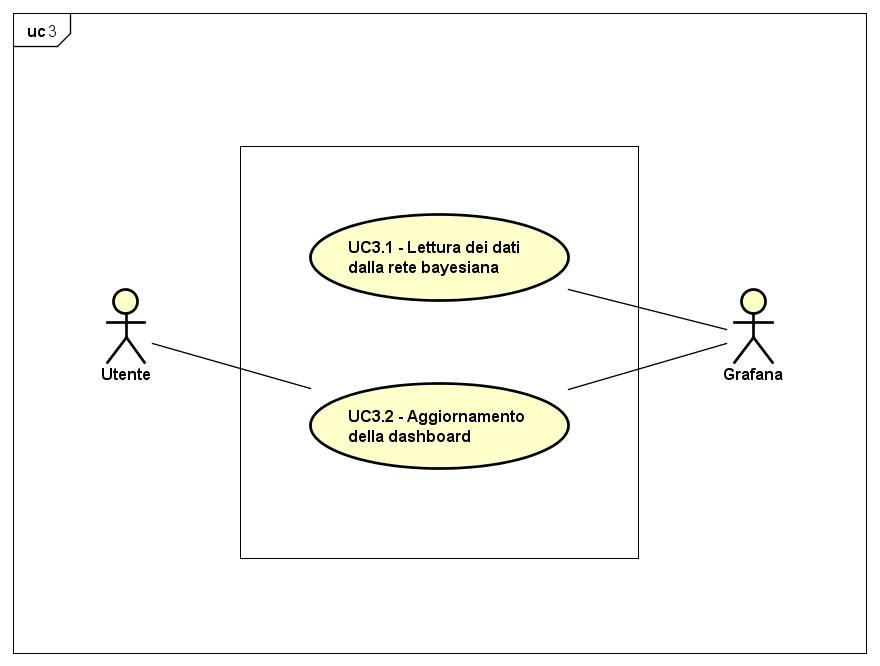
\includegraphics[scale=0.45]{Img/UC3}
	\caption{UC3: Lettura dei dati dalla rete bayesiana}\label{}
\end{figure}
\begin{itemize}
	\item \textbf{Attori}: Utente, Grafana;
	\item \textbf{Scopo e descrizione}: L'utente richiede di visualizzare dei dati calcolati dalla rete nella dashboard; Grafana legge e rende disponibili tali dati.
	\item \textbf{Precondizione}: È stata caricata e configurata una rete bayesiana adeguata; Grafana riceve correttamente informazioni dalla sorgente dati;
	\item \textbf{Flusso principale degli eventi}:
	\begin{itemize}
		\item Lettura dei dati dalla rete (UC3.2);
		\item Aggiornamento della dashboard (UC3.3)
	\end{itemize}
	\item \textbf{Postcondizione}: Grafana legge correttamente i dati dalla rete bayesiana e li rende disponibili all'utente.
\end{itemize}
\subsection{UC3.1: Lettura dei dati dalla rete}
\hypertarget{UC3.1}{}
\begin{itemize}
	\item \textbf{Attori}: Grafana;
	\item \textbf{Scopo e descrizione}: Grafana legge i dati necessari dalla rete bayesiana;
	\item \textbf{Precondizione}: Grafana riesce a leggere i dati dalla rete bayesiana;
	\item \textbf{Postcondizione}: Grafana ha letto correttamente i dati dalla rete bayesiana.
\end{itemize}
\subsection{UC3.2: Aggiornamento della dashboard}
\hypertarget{UC3.2}{}
\begin{figure} [H]
	\centering
	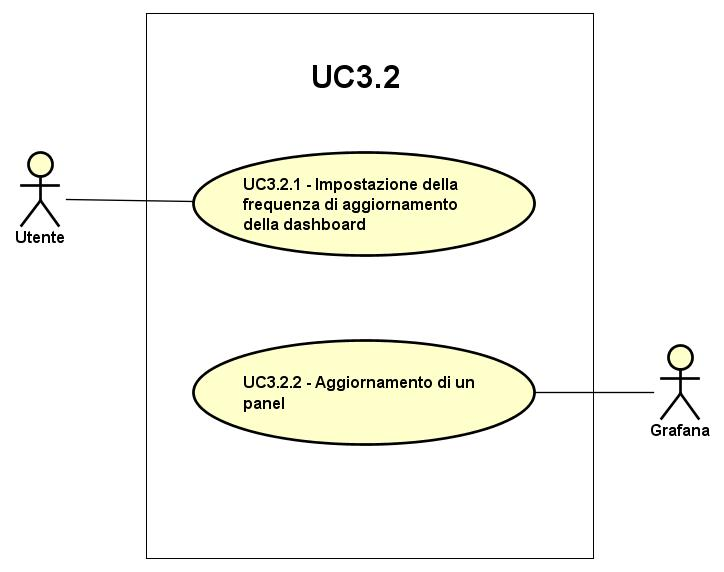
\includegraphics[scale=0.45]{Img/UC3-2}
	\caption{UC3.2: Aggiornamento della dashboard}\label{}
\end{figure}
\begin{itemize}
	\item \textbf{Attori}: Utente, Grafana;
	\item \textbf{Scopo e descrizione}: L'utente imposta la frequenza di aggiornamento della dashboard; Grafana aggiorna la visualizzazione dei panel;
	\item \textbf{Precondizione}: Grafana legge correttamente i dati dalla rete bayesiana, e il sistema permette di impostare la frequenza di aggiornamento;
	\item \textbf{Flusso principale degli eventi}:
		\begin{itemize}
			\item Impostazione della frequenza di aggiornamento della dashboard (UC3.2.1);
			\item Aggiornamento di un panel (UC3.2.2)
		\end{itemize}
	\item \textbf{Postcondizione}: Grafana aggiorna la dashboard con nuovi dati letti dalla rete, secondo la frequenza desiderata.
\end{itemize}
\subsection{UC3.2.1: Impostazione della frequenza di aggiornamento della dashboard}
\hypertarget{UC3.2.1}{}
\begin{itemize}
	\item \textbf{Attori}: Utente;
	\item \textbf{Scopo e descrizione}: L'attore imposta la frequenza secondo cui aggiornare la visualizzazione della dashboard;
	\item \textbf{Precondizione}: Il sistema permette l'impostazione della frequenza di aggiornamento della dashboard;
	\item \textbf{Postcondizione}: È stata impostata la frequenza desiderata.
\end{itemize}

\subsection{UC3.2.2: Aggiornamento di un panel}
\hypertarget{UC3.2.2}{}
\begin{itemize}
	\item \textbf{Attori}: Grafana;
	\item \textbf{Scopo e descrizione}: L'attore aggiorna la visualizzazione di un panel con nuovi dati dal flusso collegato;
	\item \textbf{Precondizione}: Grafana possiede nuovi dati relativi al flusso dati rappresentato dal panel;
	\item \textbf{Postcondizione}: La visualizzazione del panel è aggiornata in base ai nuovi dati.
\end{itemize}

\subsection{UC9: Caricamento di una rete bayesiana da file JSON}
\hypertarget{UC9}{}
\begin{itemize}
	\item \textbf{Attori}: Utente;
	\item \textbf{Scopo e descrizione}: L'attore carica la rete bayesiana da un file JSON salvato su disco;
	\item \textbf{Precondizione}: Il sistema permette di leggere un file JSON, esiste un file JSON contenente la rete;
	\item \textbf{Estensioni}:
	\begin{itemize}
		\item Viene caricato un file dal contenuto non valido e/o in un formato non valido, il sistema rimane nello stato precedente all'azione (UC2.4.1);
	\end{itemize}
	\item \textbf{Postcondizione}: La rete bayesiana viene creata secondo le informazioni salvate nel file.
\end{itemize}